\documentclass[12pt, a4paper]{article}

\usepackage[utf8]{inputenc}
\usepackage[spanish]{babel}
\usepackage{titling}
\usepackage[left=2cm,right=2cm,top=2cm,bottom=2cm]{geometry}
\usepackage{enumerate}
\usepackage{graphicx}
\usepackage{caption}

\usepackage{listings}%-para agregar codigo-
\usepackage[usenames,dvipsnames]{color}
\usepackage{color}%------------------------

%---------------------importar codigo desde archivos cpp----------------------------
\lstloadlanguages{C++}
\lstnewenvironment{code}
	{%\lstset{	numbers=none, frame=lines, basicstyle=\small\ttfamily, }%
	 \csname lst@SetFirstLabel\endcsname}
	{\csname lst@SaveFirstLabel\endcsname}
\lstset{% general command to set parameter(s)
	language=C++, basicstyle=\small\ttfamily, keywordstyle=\slshape,
	emph=[1]{tipo,usa}, emphstyle={[1]\sffamily\bfseries},
	morekeywords={tint,forn,forsn},
	basewidth={0.47em,0.40em},
	columns=fixed, fontadjust, resetmargins, xrightmargin=5pt, xleftmargin=15pt,
	flexiblecolumns=false, tabsize=2, breaklines,	breakatwhitespace=false, extendedchars=true,
	numbers=left, numberstyle=\tiny, stepnumber=1, numbersep=9pt,
	frame=l, framesep=3pt,
    basicstyle=\ttfamily,
    keywordstyle=\color{blue}\ttfamily,
    stringstyle=\color{magenta}\ttfamily,
    commentstyle=\color{RedOrange}\ttfamily,
    morecomment=[l][\color{OliveGreen}]{\#}
}

\lstdefinestyle{C++}{
	language=C++, basicstyle=\small\ttfamily, keywordstyle=\slshape,
	emph=[1]{tipo,usa,tipo2}, emphstyle={[1]\sffamily\bfseries},
	morekeywords={tint,forn,forsn},
	basewidth={0.47em,0.40em},
	columns=fixed, fontadjust, resetmargins, xrightmargin=5pt, xleftmargin=15pt,
	flexiblecolumns=false, tabsize=2, breaklines,	breakatwhitespace=false, extendedchars=true,
	numbers=left, numberstyle=\tiny, stepnumber=1, numbersep=9pt,
	frame=l, framesep=3pt,
    basicstyle=\ttfamily,
    keywordstyle=\color{blue}\ttfamily,
    stringstyle=\color{magenta}\ttfamily,
    commentstyle=\color{RedOrange}\ttfamily,
    morecomment=[l][\color{OliveGreen}]{\#}
}

\def\nbtitle#1{\begin{Large}\begin{center}\textbf{#1}\end{center}\end{Large}}
\def\nbsection#1{\section{#1}}
\def\nbsubsection#1{\subsection{#1}}
\def\nbcoment#1{\begin{small}\textbf{#1}\end{small}}
\newcommand{\comb}[2]{\left( \begin{array}{c} #1 \\ #2 \end{array}\right)}
\def\complexity#1{\texorpdfstring{$\mathcal{O}(#1)$}{O(#1)}}
 \newcommand\cppfile[2][]{
\lstinputlisting[style=C++,linerange={#1}]{#2}
}
%%------------------------------------------------------------------------------

\graphicspath{{../}}
\newcommand*\lstinputpath[1]{\lstset{inputpath=#1}}
\lstinputpath{../}

\newcommand{\subtitulo}[1]{\begin{center}\textbf{#1}\end{center}}
\newcommand{\quotes}[1]{``#1''}

\title{\textbf{Strings}}
\author{Wilmer Emiro Castrillón Calderón}

\begin{document}
	\maketitle
	
	%<*Capitulo>
	
	\section{KMP}
	\label{strings:KMP}
	
	El string matching es un problema clásico de las ciencias de la computación, consiste en buscar si una cadena de 
	texto $T$ de longitud $n$ contiene una subcadena $P$ de longitud $m$, la solución ingenua consiste en deslizar la
	cadena $P$ sobre toda la cadena $T$, comparando carácter por carácter si encajan, es decir, se empieza verificando si
	la subcadena $T[0,n]$ es igual a $P$, en caso de fallo(caracteres diferentes) se compara $T[1,n+1]$ con $P$ y así
	sucesivamente, dando como resultado una complejidad de $O(n*m)$, la cual resulta muy alta cuando los cadenas de 
	texto son muy largas.\\
	
	El algoritmo KMP(Knuth-Morris-Pratt) permite encontrar todas las apariciones de $P$ en $T$ utilizando una
	tabla de precalculo $B$
	sobre la cadena $P$, el algoritmo inicia con dos punteros, un puntero $i$ sobre $T$ y otro puntero $j$ sobre $P$,
	ambos avanzan a la par mientras se comparan $T[i]$ y $P[j]$, en caso de fallo, el cursor $j$ se devuelve a la 
	posición indicada en la tabla de precalculo($B[j]$), de esta forma solo el cursor sobre $P$ se devuelve
	y se evita devolver el cursor sobre $T$. El algoritmo KMP se divide en dos partes, una primera para calcular la 
	tabla de precalculo $B$ y una segunda para aplicar la búsqueda de $P$ sobre $T$.\\
	
	La tabla de precalculo consiste en buscar la longitud de los \quotes{bordes} de $P$, un borde se define como un 
	substring que es prefijo de $P$ y sufijo de un substring $P[0,k]$, entonces $B[k+1]$ es igual a la longitud
	del borde del substring $P[0,k]$, por ejemplo en la figura \ref{strings:KMP:bordes} se observa el
	borde para $P$ = \quotes{ABRACABRAABRA}, se recomienda hacer el proceso a mano para que se pueda entender mejor.
	
	\begin{figure}[!htb]
		\centering
		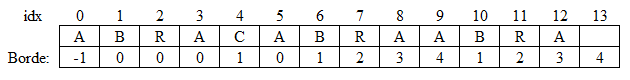
\includegraphics[scale=0.9]{strings/imagenes/KMP/bordes}
		\caption{}
		\label{strings:KMP:bordes}
	\end{figure}
	
	Para el proceso de buscar las repeticiones de $P$ sobre $T$ se necesitan dos punteros como se había mencionado 
	antes, el puntero $i$ sobre $T$ y $j$ sobre $P$, observemos la figura \ref{strings:KMP:match1}, los punteros 
	avanzan hasta llegar a al indice $9$, donde hay un carácter de fallo, en este punto se puede observar la mejora
	que ofrece el KMP, pues solamente se devuelve $j$ a la posición $B[j]$ para seguir comparando, como se observa
	en la figura \ref{strings:KMP:match2}.\\
	
	\begin{figure}[!htb]
		\centering
		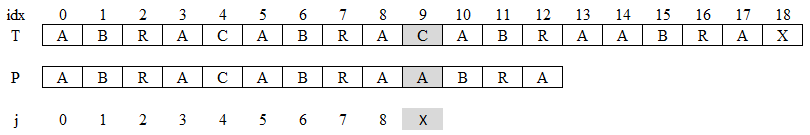
\includegraphics[scale=0.75]{strings/imagenes/KMP/match1}
		\caption{}
		\label{strings:KMP:match1}
	\end{figure}
	
	\begin{figure}[!htb]
		\centering
		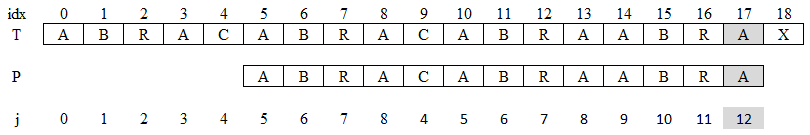
\includegraphics[scale=0.75]{strings/imagenes/KMP/match2}
		\caption{}
		\label{strings:KMP:match2}
	\end{figure}
	
	La implementacion no es larga y consiste en realizar primero la búsqueda de los bordes de $P$ y posteriormente 
	hacer la búsqueda de $P$ sobre $T$. El algoritmo resultante tiene complejidad $O(n+m)$.
	
	\cppfile[7-28]{strings/codigos/KMP.cpp}
	
	El KMP puede encontrar repeticiones con intervalos cruzados, por ejemplo con $P$ = \quotes{ABCABC} y 
	$T$ = \quotes{DABCABCABCD}, hay 2 repeticiones, en los rangos $(1,6)$ y $(4,9)$, en este caso se cruza el rango 
	$(4,6)$ el cual aparece ambas repeticiones. Si no se requieren intervalos cruzados se puede simplemente reiniciar
	el puntero $j$ a $0$ al encontrar cada repetición (linea 19 del código), de esta manera se continuará buscando 
	desde el inicio de $P$.
	
	%si $b[j]>0$ se garantiza que la subcadena $P[0,B[j]-1]$ es igual a la subcadena $T[i-b[j],i-1]$
	
	%</Capitulo>
	
\end{document}


